% !TeX root = ../main.tex

\chapter{Phase match condition for spontaneous four wave mixing in a ring cavity }\label{chap:pmc-sfwm}

According to the previous chapter, in a typical nonlinear optical waveguide or silica fibers, despite the stimulated Raman and Brillouin scattering, the frequency conversion processes involve not only the self-phase modulation of pump light and cross-phase modulation of signal and idler light, but also the phase mismatch in four wave mixing propagation factor. 
%\begin{equation}\label{key}
%	\Delta \phi = \Delta_M
%\end{equation}
In this case, it is necessary to study the coupled nonlinear equations involving signal, idler and pump intensity \cite{AGRAWAL2013397}. 

Whereas in ring resonators, whose mode linewidth (pm) is much narrower than self-phase modulation frequency broadening, 
the frequency broadening in single mode is negligible. 
Thus the phase mismatch among cavity modes becomes the critical factor of the band of four wave mixing.

This chapter first describes the major origin of phase mismatch, chromatic dispersion, and goes on to the design philosophy used in device fabrication. Besides, several topics concerning the band of phase matching are also included.

\section{Chromatic dispersion}

In a typical FWM process, both energy conservation and momentum conservation are required 
\begin{align}
  \beta_i + \beta_s & = 2 \beta_p \label{eq:beta-cons} \\
  \omega_i + \omega_s & = 2 \omega_p \label{eq:omega-cons}
\end{align}
where the subscripts $s~i~p$ stand for signal, idler and pump light.

Meanwhile, the resonance condition \autoref{eq:res-con} leads to $\beta = m \frac{2 \pi}{L}$. Thus, \autoref{eq:beta-cons} is equivalent to 
\begin{equation}\label{eq:mu-cons}
  m_i + m_s = 2 m_p 
\end{equation} 
  
We can see that \tmtextit{the momentum conservation agrees with mode number
conservation.} That is to say, as pump light sets into resonant wavelengths, by choosing the equidistant modes relative to the pump mode, the momentum conservation can be naturally satisfied. This is the most important difference from non-resonant devices.

Therefore, we can estimate the phase mismatch only in the frequency domain. Expand the resonant frequency into Taylor seires at $\omega_0$ to the propagation constant $\beta$
\begin{eqnarray}\label{eq:omega-taylor}
  \omega_{\mu} & = & \omega_0 
  + \sum_{j=1}\dv[j]{\omega}{\beta} (\beta_{\mu}-\beta_0) \frac{{(\beta-\beta_0)}^j}{j!} \\
  & = & \omega_0 
  + \sum_{j=1}\dv[j]{\omega}{\beta} \qty(\frac{2 \pi}{L})^j \frac{\mu^j}{j!} \nonumber \\
  & = & \omega_0 + D_1 \mu + \frac{D_2}{2!} \mu^2 + \frac{D_3}{3!} \mu^3 + \cdots \nonumber
\end{eqnarray}
where $D_j \equiv  (\frac{2 \pi}{L})^j\dv*[j]{\omega}{\beta}$ are \textit{j}-order mode number dispersion parameter, whose dimension are all $\mathrm{T}^{-1}$ and $\mu \in \mathbb{Z}$ is the relative mode number. 

It is easy to know that $D_1 / 2 \pi = v_g / L$ is the free spectral range in the frequency and indicates that the dispersion property is related with the difference of resonant frequencies.   

Next, we introduce the integrated dispersion $\dint$ \cite{Brasch2014a} to analyze the phase mismatch
\begin{align}\label{eq:def-dint}
    D_\mathrm{int}(\mu) &\equiv \omega_{\mu} - (\omega_0 + D_1 \mu)  \\
    &= \frac{D_2}{2!} \mu^2 + \frac{D_3}{3!} \mu^3 + \cdots \nonumber
\end{align}

In particular, $\dint$ is the residual dispersion higher than second order. Approximately, if $D_3 \mu \ll D_2$, the second-order dispersion will dominate the integrated dispersion both at signal and idler mode.

Indeed, the mode number dispersion parameter is linked with the dispersion coefficients in frequency and wavelength domain, giving such a chain rule
\begin{equation}\label{eq:disp-chain}
    D_2 = - \frac{L}{2\pi} {D_1^3}{\beta_2} = \frac{L}{2\pi}  \frac{\lambda^2}{2\pi c} {D_1^3} D_{\lambda}
\end{equation}
where $\beta_2=\dv*[2]{\beta}{\omega}$ is group velocity dispersion (GVD) and $D_{\lambda}= - (\lambda/c)\dv*[2]{n}{\lambda}$ is the dispersion parameter.

In this method, we can analyze the phase mismatch in FWM quantitatively
\begin{align}\label{eq:freq-mismatch}
	\Delta \omega &\equiv \omega_s + \omega_i - 2 \omega_p \\
%	&=  D_{\mathrm{int},s} + D_{\mathrm{int},i} \\
	&= \dint(\mu) + \dint(-\mu) \nonumber \\
	&= 2\qty(\frac{D_2 \mu^2}{2!} + \frac{D_4 \mu^4}{4!} + \frac{D_6 \mu^6}{6!} +\cdots)  \nonumber
\end{align}

From the above derivation, the frequency mismatch $ \Delta\omega $ only adds to the even terms of Taylor series in \autoref{eq:omega-taylor}.
To conclude, a rough presupposition to increase the efficient phase matched band is achieving zero and flat dispersion around pump wavelengths.

\section{Dispersion compensation}\label{sec:disp-comp}
Previously mentioned  in \autoref{sec:guide}, the dispersion behaviour in integrated devices is not only the intrinsic material property, but also depends on the waveguide dimension. 

In other words, the phase mismatch occurs as a result of material dispersion $D_M$ and waveguide dispersion $ D_W $, $D_{\lambda}= D_M + D_W$. Here, we adopt the wavelength dispersion parameter since the wavelength domain is measurable.

Usually, the Sellmeier equation is used to fit the refractive index for a particular transparent medium based on the Lorentz-Drude mode. \citeauthor{Luke2015a} reported the below measured refractive index of stoichiometric \ce{Si3N4} film \cite{Luke2015a}
\begin{equation}\label{eq:si3n4-selleimeier}
    n_{\ce{Si3N4}}^2 = 1 + \frac{3.0249 \lambda^2}{\lambda^2-135.3406^2} + \frac{40314 \lambda^2}{\lambda^2 - 1239842^2}
\end{equation}

This Sellmeier equation is valid over the wavelength range 310–5504 \si{\nm}.
The result of \autoref{eq:si3n4-selleimeier} is plotted in \autoref{fig:Luke-si3n4}, along with the material dispersion parameter $D_M$, which is calculated at the precision of \si{\nm} using the second-order finite difference of refractive index. In the telecom C-band, $n$=1.9963 and $D_M$ = -6.57 \dispu, which suggests the material dispersion at this range is considerably small.

\begin{figure}
    \centering
    \includesvg{luke/Luke}
    \mycaption{Refractive index and dispersion parameter measured in reference}{$ \lambda$=1550 \si{\nm}, $n$=1.9963 and $D_M$ = -6.5656 \dispu .}
    \label{fig:Luke-si3n4}
\end{figure}

On the other hand, the numerical simulation is adopted to evaluate the waveguide parameter.
We use commercial software \si{\nm}{Lumerical MODE} to solve for the refractive index of fundamental TE modes.
Shown in \autoref{fig:wg-disp}, the dimension dependence of waveguide dispersion features negative values in the small waveguide size, i.e. behaving as normal dispersion at the second order. Nevertheless, as either the thickness or width of channel waveguide increases,
$D_W$ turns positive. This indicates that to achieve zero dispersion in phase match condition of four wave mixing, the normal material dispersion can be compensated with anomalous waveguide dispersion. 

For example, at 1550 \si{\nm}, in a 1.5-\si{\um}-wide and 0.8-\si{\um}-thick silicon nitride waveguide cladded by silica, where the refractive index is 1.48,
the waveguide dispersion is 45 \dispu. Substituting into the second-order dispersion chain rule in \autoref{eq:disp-chain}, the second-order mode number dispersion parameter $ D_2 $ is about 12 kHz. It is close to zero dispersion for the pump wavelength.

\begin{figure}
	\centering
	\includesvg{wg_disp/fdtd_fine}
	\mycaption{Waveguide dispersion map simulated by Lumerical MODE}{The central wavelength to perform the simulation is 1550 \si{\nm} and the precision is nm. We select the fundamental TE mode as the objective to study the waveguide dispersion. The scattered point in the figure is 1.5-\si{\um}-wide and 0.8-\si{\um}-thick.}
	\label{fig:wg-disp}
\end{figure}

\section[{Dispersion engineering using slot structure}]{Dispersion engineering using \\ slot structure}

The slot waveguide was firstly realized by \citeauthor{Xu2004} experimentally \cite{Xu2004}. The same group, \citeauthor{Almeida2004} then discussed the light enhancement and confinement caused by large discontinuity of the electric field at high-index-contrast interfaces \cite{Almeida2004}. In the recent decade, it is fully studied that such a novel waveguide can be also used to design dispersion-flattened waveguide \cites{Mas2010, Zhang2010, Zhu2012, Nolte2013}, including the both vertical or horizontal and single or multiple slots. It is also reported a micro-ring resonators formed by a slot hybrid waveguide 
exhibits a flat and low anomalous dispersion \cite{Zhang2013}.

In our research, the vertical slot is preferred due to the easy fabrication during the monolithic process. 
%We propose a double-slot silicon nitride to achieve near-zero and flat dispersion.
For example, in a double vertical slot waveguide illustrated in \autoref{fig:slot-illus}, two extra gaps are fully etched and then reburied with low-index medium instead. 
Except the waveguide width $w$ and thickness $t$, two extra parameters are defined, the position factor $ \mathit{pf} $, ratio of slot position to the waveguide width $w$, and the filling factor $ \mathit{ff} $, ratio of slot width to the waveguide width.

\begin{figure}
		\centering	
		\includesvg[width=3in]{slot/slot_illus}
		\mycaption{Illustration of a double vertical slot waveguide}{The cyan region is \ce{Si3N4} waveguide and surrounded by silica.}
		\label{fig:slot-illus}
\end{figure}


\begin{figure}
	\centering
	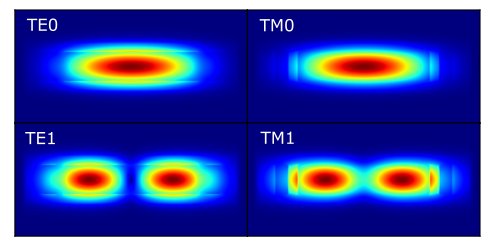
\includegraphics[width=.8\linewidth]{imgs/png/slot_mode}
    \mycaption{Modes of the double vertical slot waveguide}{$w$=2.5, $t$=0.8, $\mathit{ff}$=0.053, $\mathit{pf}$=0.4}
 	\label{fig:slot-mode}
\end{figure}

%\begin{figure}
%	\centering
%	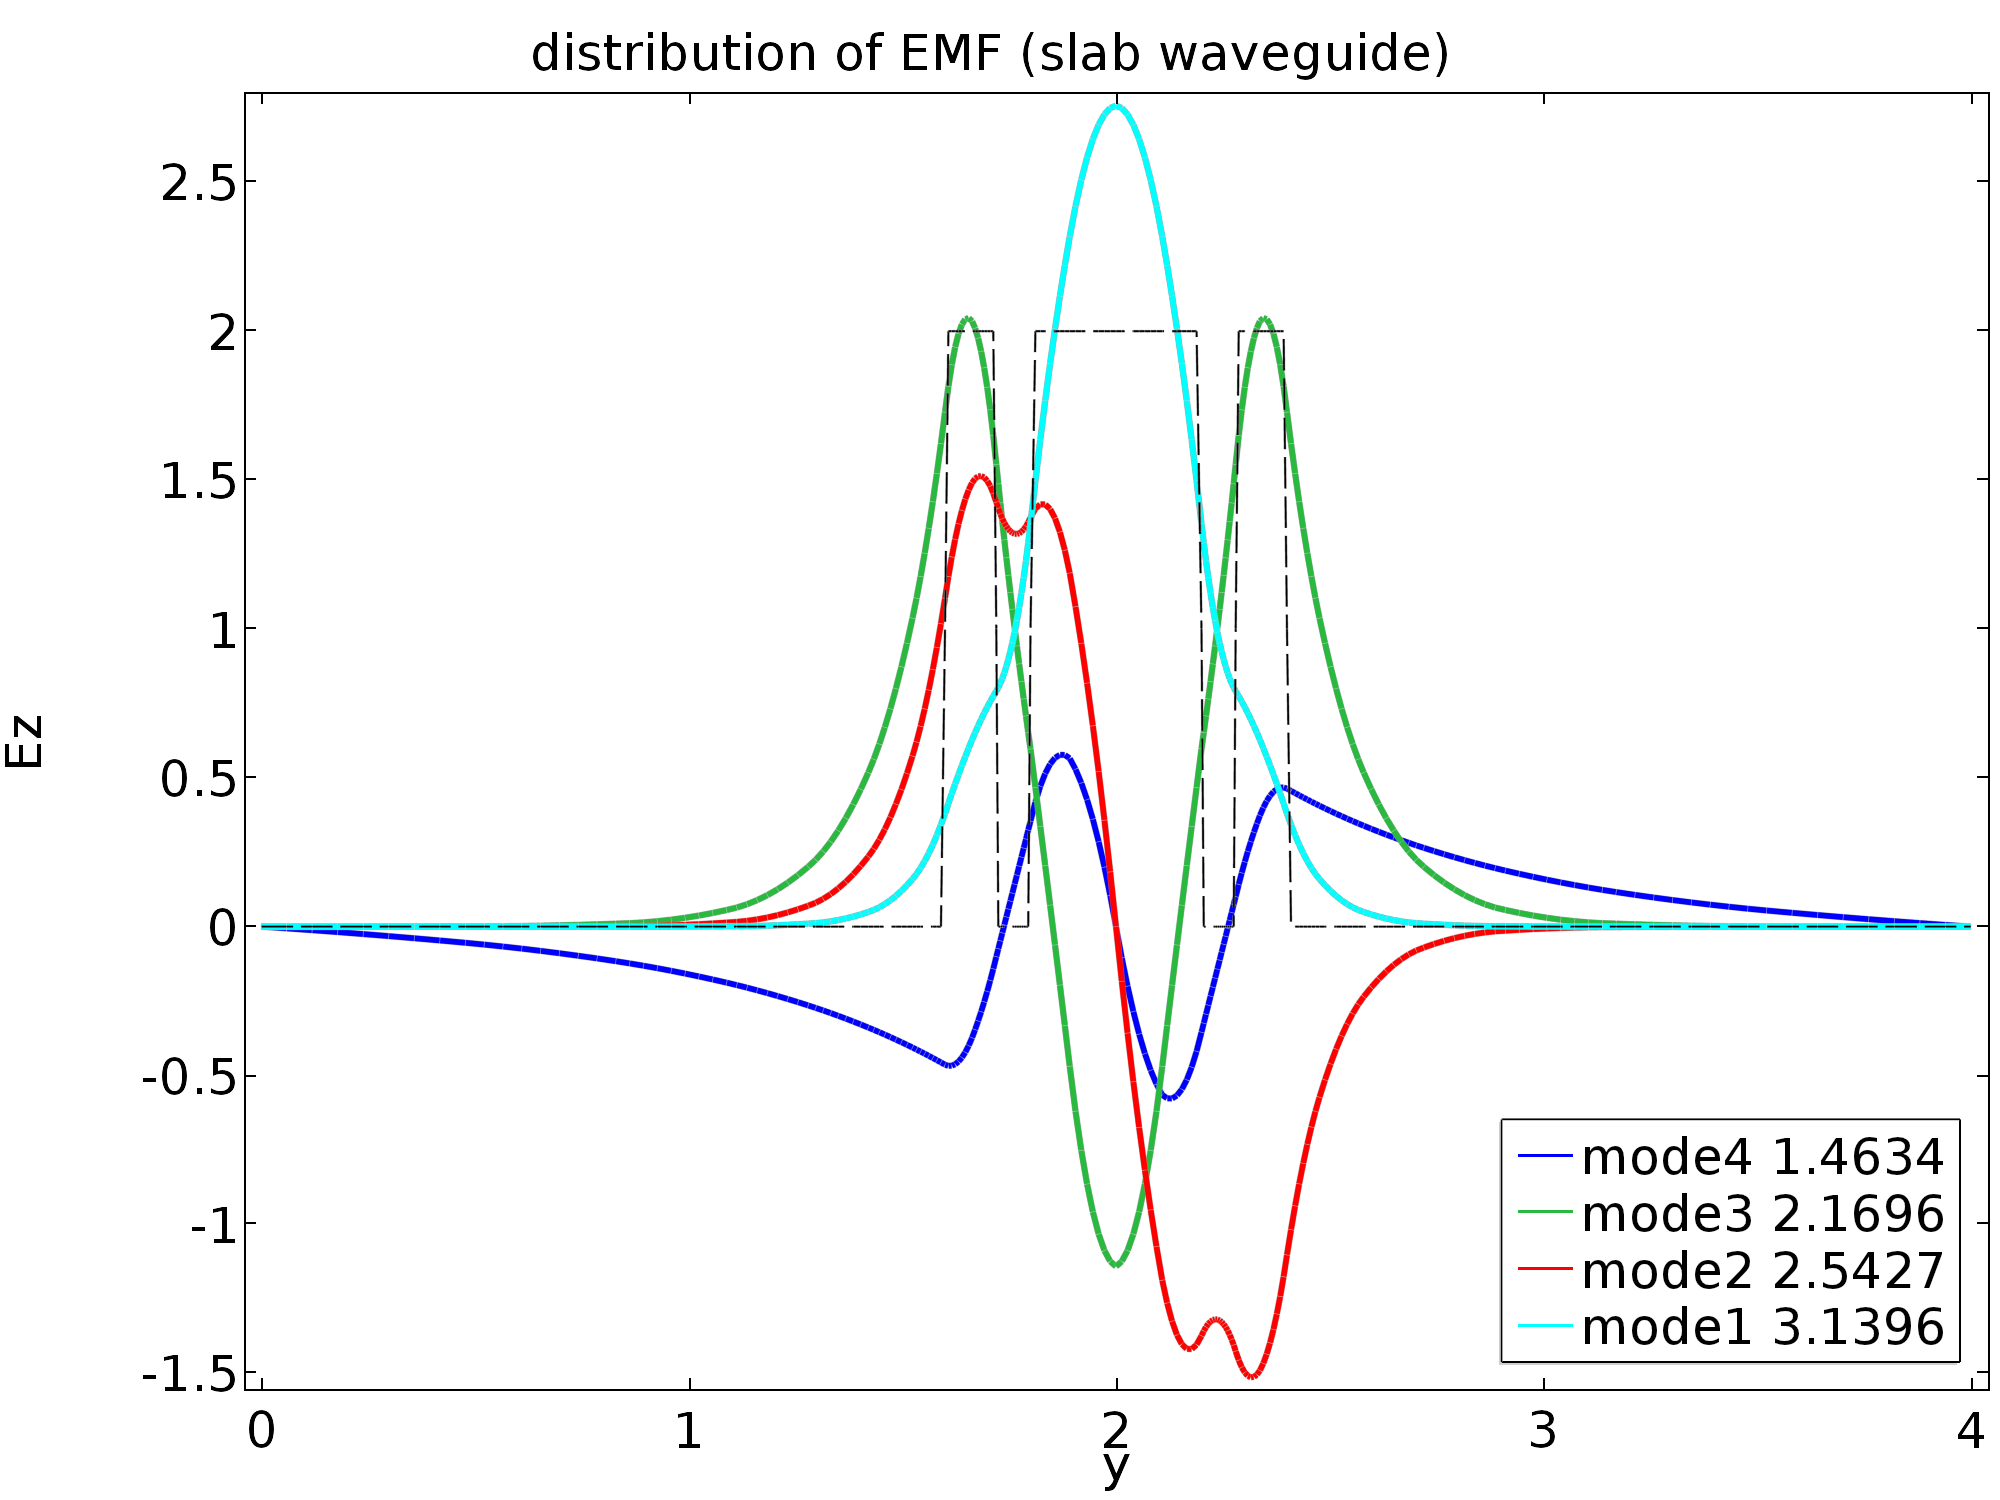
\includegraphics[width=0.7\linewidth]{imgs/png/Ez}
%	\mycaption{Modes of the double vertical slot waveguide}{}
%	\label{fig:slot-mode-Ez}
%\end{figure}

To classify the modes in this slot structure, the same mode solver mention in previous section is performed.
In the result shown in \autoref{fig:slot-mode}, in TM0 and TM1 modes, the light is confined strongly in the slots while the TE0 and TE1 is similar to the normal TE modes, where the discontinuity is obvious on the upper and lower interfaces.

%An interesting finding is that differing from the simple rectangular waveguide, 
%the mode of both quasi-TE and quasi-TM modes can be assumed as the symmetric and anti-symmetric combination of the mode field on both sides. 

%\begin{align}\label{key}
%	\vb{E}_\mathrm{sym} &= \vb{E}_{l} + \vb{E}_{r} \\
%	\vb{E}_\mathrm{asym} &= \vb{E}_{l} - \vb{E}_{r} \nonumber
%\end{align}

%\autoref{fig:slot-mode-Ez} is the \textit{z}-component of the electric field of the four modes. For example, quasi-TE0 mode is even parity while quasi-TE1 mode is odd parity.

Furthermore, by optimizing the position and filling factors, the near-zero and flattened dispersion can be obtained. 


\section{Effects of mode crossing}

In the conclusion of \autoref{sec:disp-comp},
only in the wider or thicker waveguides can the zero dispersion be compensated. However, 
despite the fabrication difficulty arising from thicker films,
the waveguide of larger size also supports high order modes. 

In this case, due to the perturbation of high order modes, the linear mode coupling occurs and influences the resonance spectrum. 
In the study of soliton generation,
it is found that avoided mode crossings induced by linear mode coupling can prevent optical soliton formation when affecting resonator modes close to the pump laser frequency \cites{Herr2014a,Bao2018}. On the other hand, by introducing artificial mode crossing, the anomalous group velocity can also be achieved \cite{Kim2017}. Even though the phenomena mentioned in these works are classical, but in the term of phase matching condition, the physics is similar.

In the following research, the mode crossings found in our devices not only change the spectrum transmission, but also leads to failure of evaluating the dispersion properties.



